\chapter{绪论}
\section{研究背景及意义}
人类处在一个三维的世界环境中,我们所认识的事物无一不是一个三维的构成的现实物体。人类开展的各种科学研究,都是针对人类所面临的各种科学问题,各种现实问题。这些科学研究有的关于现实世界的感知,有的关于现实物体识别与构建。目前各种智能设备风起云涌,3D场景构建更是炙手可热。这些设备可以对三维场景进行感知,并且模拟出真实的3D场景,从而帮助人们能够在此基础上进行更加高级的运用。例如,虚拟现实技术,无人机、机器人的自主导航技术等等。自动驾驶汽车就是该领域的突出代表,如图\ref{fig_1-1}所示。自动驾驶技术突破了场景识别、场景解析、三维物体识别、三维地图构建、地图构建与定位技术(SLAM)等。

\begin{figure*}[tb]
\begin{center}
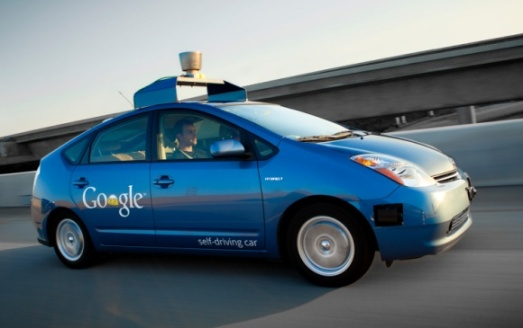
\includegraphics[width=0.4\linewidth, height=5cm]{figures/1-1a.jpg} 
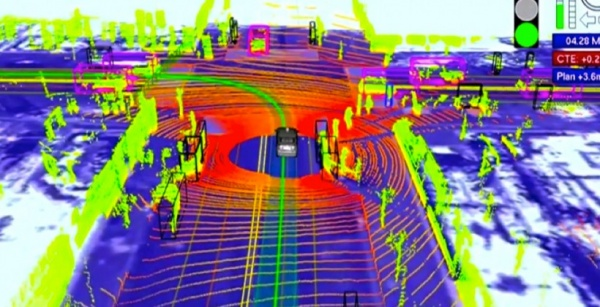
\includegraphics[width=0.4\linewidth, height=5cm]{figures/1-1b.jpg}
\end{center} 
\vspace{-4mm}
\caption{Google自动驾驶汽车和其场景感知的示意} \label{fig_1-1}
\end{figure*}

\begin{figure}[tb]
\begin{center}
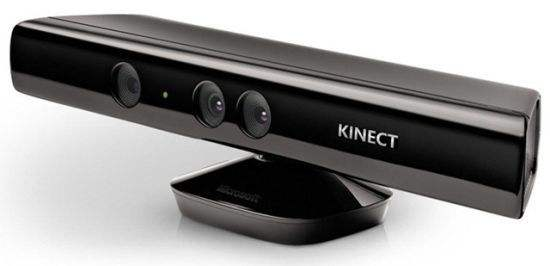
\includegraphics[width=0.4\linewidth]{figures/1-2.jpg} 
\end{center} 
\vspace{-4mm}
\caption{微软发布的首款RGB-D设备Kinect} \label{fig_1-2}
\end{figure}

近年来,业界对三维模型的研究是如火如荼,
%三维模型因为其丰富的形状、颜色、纹理等信息,在多媒体,图形学,虚拟现实,设计,娱乐,工业制造等领域得到了越来越广泛的应用
在工业设计、图形学、虚拟现实等方面被广泛应用\cite{Tangelder2008A}。三维数据库已经硕果累累。同时3D打印技术的出现,使得三维形状模型的应用更加实用化,这种增材制造技术能够完成许多传统减材制造技术所不能完成的复杂产品生产。除此之外,谷歌的Kinect等性价比高的RGB-D设备如图\ref{fig_1-2},更加丰富了三维模型的来源。为了在三维形状的匹配,查找和分类等方面获得优秀的表现,我们需要高效准确的图形检索、分类的方法来处理这些海量三维数据。

三维形状模型与一般的二维图像相比,更丰富真实、更好的符合了人类视觉特性、能够更加清楚的表示现实世界的物体。一般情况下三维形状模型由网格数据结构,包括顶点、面、边等基本数据来表述,因此具有相对复杂的数据结构,与声音、图像相比更加难以处理。三维模型在三维扫描技术与设备以及交互建模技术的发展下迅速增加,方便了研究者的就一步的探索。但由于三维模型较其他类型的数据结构相比复杂,目前仍然存在一些难以解决的问题:前期的三维形状建模工作已经非常成熟,免去了研究者亲自建模的烦恼,可是迅速的识别与检索技术仍然有待解决。另外三维形状匹配还可以在以下领域得到广泛的应用,机器人或无人飞行器通过三维形状匹配在数据库中快速地检索并识别物体,用来寻找并确定目标或者用来躲避障碍物,提高其自身的智能程度;公共安全等领域利用三维匹配技术来查询二维或三维人脸库、三维头颅库等匹配相关信息,能够大大降低恐怖袭击和刑事犯罪对社会的危害;工业现场可以根据图像或图形匹配自动判定控制信息、故障类型等;在生物医学方面,由CT、MRI、PET等断层成像设备产生了大量的三维数据,如何准确快速地查找并处理这些信息,对于提高诊断的准确率并提高我国医疗健康水平,缓解人口老龄化带来的压力至关重要。

传统的三维形状分析技术就是设计出优秀的三维形状特征,这些三维形状特征来自颜色、纹理、形状等不同的属性,能够有效的应对三维形状的分类任务。目前大量用于描述三维模型的特征被提出,例如:平均测地线距离 (Average Geodesic Distance),Si-HKS (Scale-invariant Heat Kernel Signature),SDF (Shape Diameter Function)等,这些特征虽然有一定的效果,但是同时具有一定的局限性。局限一:传统方法的特征要求设计人员具有较强的专业知识和优秀的数学功底;局限二:传统方法的特征针对性很强,即特征只针对某个属性,三维形状的其他信息在提取过程中丢失严重,影响了识别效果。


同时三维形状内容的匹配与检索没有像文本内容匹配与检索那样简单,因为从一篇文章中提取若干关键文字信息,或从一幅图像、一段视频中提取能够代表该图像的描述信息,三维形状的数据结构存在拓扑等复杂结构,因此处理相对复杂,已研究出的特征提取、匹配与检索方法仍存在一定的局限性,因此目前只有具有高级思维的人类才可以完全实现。通过计算机提取多媒体信息的特征仍然是一件困难的事情,也是多媒体匹配与检索的核心技术之一\cite{Tangelder2008A, Funkhouser2005Shape}。三维模型匹配、对齐、分割中,形状特征的提取是非常关键的技术之一,提取的形状特征需要有如下特点:1)良好的类间可分性和类内相似性,用以保证形状描述的准确性;2)对形状变形不敏感,尤其非刚性变形; 3)尽可能低的特征维数,和能够表示三维形状的显著特征,这样就能减少搜索或者匹配的计算量,大大提高计算性能。


%%%%%%%%
%%  \upcite{} 可以使引用变为上标
%%

\section{三维模型的研究状况}

\subsection{国外现状分析}
国外对三维形状识别研究起步较早,研究者主要关注于整体特征的提取,已经获得了大量的研究成果\cite{Tangelder2008A,Funkhouser2005Shape,Krizhevsky2017ImageNet,Kaick2010A,Ullman1985Three, Loncaric1998A, Campbell2001A}。美国Carnegie Mellon大学的Johnson等人\cite{Johnson2002Using}提出了一种经典的局部描述符 Spin Image,该描述符将临近的顶点投影到了一个二维的柱面坐标下,因此复杂的三维形状匹配转化成了相对简单的二维图像的匹配。该方法具有很强的鲁棒性,但这个方法中需要计算并匹配每个顶点的spin image,因此计算效率不高,此外该特征描述符无法很好的应对非刚性变形。之后美国Sarnoff公司的Shan等人\cite{Shan2006Shapeme}提出了使用Shapeme投影的方法来分割需要匹配的形状,从而加速形状匹配的速度; Liu等人\cite{Liu2006Shape}提出了使用Monte Carlo稀疏采样的方法来降低计算量,并使用k-means方法使得到的数据量得到有效的降低从而提高匹配速度。另外希腊Centre for Research and Technology Hellas的Malassiotis等人\cite{Malassiotis2007Snapshots}提出了Snapshot局部特征描述符,该描述符能够很好应对自身的重叠以及假象的影响,并且该方法使用更高效的特征对齐方法,能够获得很好的性能,但仍然无法很好的应对非刚性变形。

大多数情况下,对象物体不仅仅含有刚性变形,还具有非刚性变形,例如弯曲、姿势改变、局部形状变化等。这种变形过程中任意两点测点距离不变,即称之为等距变形。研究者着眼于非刚性形变也做出了巨大贡献。美国ioIMAGE公司的Elad等人\cite{Elad2001Bending}首先在这方面做了尝试,他们根据形状弯曲变形中表面上的长度并未发生变化这一特点,利用MDS(Multidimensional Scaling)完成了测地线距离与欧式距离的转换,相当于复杂的非刚性变形的转化成了简单的刚性形状。之后美国Stanford大学的Emoli等人\cite{M2005A}与以色列的Israel Institute of Technology大学的Bronstein等人\cite{Bronstein2006Efficient}扩展了这项研究,他们使用Gromov-Hausdorff距离来计算形状的相似程度,这样能够有效的降低两个形状建立对应关系时所产生的误差。由于这类方法基于高计算复杂度的最优化方法,因此只能适用于一对一,或者一对少数形状的匹配。德国University of Hannover的Reuter等人\cite{Reuter2006Laplace}尝试使用Laplace-Beltrami谱作为等距变形的形状描述符,这个描述符具有更小的计算复杂度,因此最近受到很大的关注。Wu等人\cite{Wu2010Global}扩展了这个方法,在他们的研究中使用随机采点的方法得到一定数量的顶点,在每个顶点附近选择一个局部区域,选择方法是使用固定面积比率的方式,然后计算该局部区域的Laplace-Beltrami谱,然后与全局的Laplace-Beltrami谱进行结合,这样兼顾了全局和局部特征,因此获得了更好的性能。美国Stanford大学的Sun等人\cite{Sun2009A}提出了HKS(Heat Kernel Signature: HKS)的描述符,通过求解每个顶点的热扩散方程,求取基础解-热核作为局部特征。其优点在于选择不同的扩散时间可以控制所包含的局部范围。该方法只需要特征分解拉普拉斯系数矩阵,效率较高,弱点在于不能应对尺度变换和拉伸变换。以色列的Israel Institute of Technology大学的Bronstein等人\cite{Bronstein2010Scale}改进了热核特征描述符,使之能够应对形状的尺寸变形的影响。

另外一方面,由于三维形状的各个部分的重要程度不同,因此利用区域的重要程度来选择需要匹配的顶点或区域能够极大地降低计算复杂度并提供形状对应、匹配、与检索的速度。首先是美国Maryland大学的Lee等人\cite{Lee2005Mesh}提出了对高斯加权平均曲率做center-surround的网格显著区域提取的方法,通过实验得知该方法能够捕获网格上绝大多数的显著区域,但该方法的缺陷是得到的显著区域过于稀疏,导致形状匹配精度的下降。之后,美国Princeton大学的Shilane等人\cite{Shilane2007Distinctive}提出另一种形状显著区域提取的方法,任意一个给定顶点对已建立的数据库进行检索,使用DCG(discounted cumulative gain)值来进行该点附近的显著区域检测,若使用该区域检索能够获得高的DCG值,则表明该区域是重要,反之则认为是普通的区域相对不重要。该方法能够提供更高精度的局部显著指标,然而这个方法由于计算量大,并且需要事先构建一个形状数据库,因此比较难以在实际中应用。波兰Institute of Theoretical and Applied informatics of PAS的Glomb\cite{G2009Detection}将图像领域的Harris运算符扩展到了三维领域,通过计算顶点附近区域的形状变化来衡量该点局部区域的显著程度。法国INRIA Grenoble Rhone-Alpes的Zaharescu等人\cite{Zaharescu2009Surface}将图像领域内知名的DOG(Difference of Gaussians)方法在三维形状方面进行了尝试,并提出了Mesh DOG方法,该方法具有对方向、旋转、平移和缩放具有较高的鲁棒性,但仍然不能很好的应对非刚性变形。

由于三维形状的匹配与检索相对复杂,很难推导出理论的评价方程,因此常常使用标准形状库来评价各种方法。美国Princeton大学的Shilane等人\cite{Shilane2004The}提出一套三维模型库Princeton Shape Benchmark,该数据库包含了1814个通用物体模型,并分成了训练和测试两组。加拿大McGill大学Siddiqi等人\cite{Siddiqi2008Retrieving}提出了专门针对关节变形物体的形状标准库McGill 3D Shape Benchmark。以色列Israel Institute of Technology大学的Bronstein等人\cite{Bronstein2009Numerical}设计并制作了专门针对非刚性变形的形状标准库TOSCA,可供部分匹配和检索研究之用。美国国家标准与技术研究院提出的SHREC2011非刚性变形形状库\cite{Lian2011SHREC},包含600个非刚性变形的物体,适合包含非刚性变形方面的分析与评价

\subsection{国内现状分析}

国内在三维形状特征描述符方面起步较晚,研究主要集中在全局特征描述符上,经过近几年的努力取得了可喜的研究成果。刘等人\cite{刘志2016基于特征线条的三维模型检索方法}为了避免在三维模型检索中对输入源的限制,提出一种以自然图像为输入源、基于特征线条的三维模型检索方法。黄等人\cite{黄骥2016基于核线性分类分析的三维模型检索算法}为提高检索精确度,提出了一种利用核线性分类分析来对模型特征进行优化的新方法。张等人\cite{张全贵2017融合}针对手绘草图检索三维模型时存在的表达模糊性和绘制随意性等问题,提出基于Fuzzy拓扑关系与角点典型形状上下文(CRSC)的三维模型检索方法。李等人\cite{李闯2016基于平均自旋图的三维形状特征描述}基于自旋坐标和自旋图理论,给出基于平均自旋图的三维形状特征描述方法,用于三维模型检索。周等人\cite{周燕2016基于多特征融合的三维模型检索算法}针对三维模型检索中单一特征检索效果差的难题,首先提出了三维模型的3类特征向量提取算法,即刻画模型表面特性的扩展高斯球面特征向量、反映模型内部结构的Radon变换球面分布特征向量、代表模型投影层次的视图分层压缩感知特征向量。其次,以样本模型的查询结果分类信息熵作为指标并结合监督学习过程,给出了一种多特征融合的加权系数估算方法。

\section{深度学习技术}

深度学习(Deep Learning)由于其出色的表现,逐渐使得其成为研究的热点。针对深层次网络训练的难题,人们提出了BP算法\cite{Rumelhart1988Learning}。BP算法是深度学习的基础算法之一。Yann LeCun等\cite{Lecun2014Backpropagation}提出了卷积神经网络(Convolutional Neural Network)使人们看到深度学习的巨大潜力。然而,能够训练的网络深度只有两到三层,严重抑制了深度学习的发展进步。事情的转机出现在2006年,由于深度置信网络模型(DBN)的巨大突破,使得深度学习开始产生。Hinton等人\cite{Hinton2006A}使用贪婪算法对网络参数进行自底向上进行逐层预训练,由此可对前馈网络模型进行预训练。
%
随着深度学习技术不断发展,大量的新的深度学习算法被提出。其中比较出色的包括自动编码器(AutoEncoder)、卷积神经网络(CNN)、循环神经网络(RNN)、深度神经网络(DNN)、深度玻尔兹曼机(DBM)、卷积深度置信网络(CDBN)等等。2012年,Alex等人利用卷积神经网络设计的算法在Imagenet图像识别竞赛中表现优秀\cite{Krizhevsky2017ImageNet},在后续图像各方面的研究中,这种类型的卷积神经网络都已经被广泛采用。而在声音识别领域,百度公司采用深度学习方法研发出的语音识别系统Deep Speech,也能取得非常好的识别效果\cite{Niu2014Context}。

近年随着深度学习算法的深入研究,深度学习算法已经深入到IT领域的各个方面,各个互联网巨头都不惜重金,发展深度学习,例如腾讯的DX-I框架,阿里巴巴的PAI2.0框架。Google的Deepmind团队的AlphaGo更是在围棋方面战胜世界一流棋手李世石。不久前更是推出了``最强版”AlphaGo Zero。深度学习已经是目前的风口浪尖,其能够通过学习的方式得到表达能力更强的阶层式特征,并对海量数据进行处理,因此深度学习的方法可以应用于三维形状的识别问题。一般的特征包括颜色的直方图,纹理的直方图,Gist,HoG, SIFT, SURF等,尽管这些特征在某些应用中取得了比较理想的效果,但是它们只能刻画图像当中某一方面的信息,也就是说这些特征在不同的任务中,效果并不都是最优的。
%
最近几年越来越多的研究表明,特征的提取和分类是相互交织在一起的,通过学习方式得到的特征能够获得更高的性能。图像信息在人类理解和认知外界环境中起到主要的作用,将图像信号经过人脑视觉系统处理之后,我们能够对物体进行识别、对场景进行理解,从而使得我们能够对环境做出反应。但是,为什么人脑有如此强大的信息处理能力,从而让我们在短时间之内对环境做出非常准确的理解与判断?以及怎样才能让机器模拟人的大脑视觉系统处理图像?神经生物学家、生物医学家对人脑进行研究发现大脑的视觉系统处理是一种“分层学习” 机制,如图\ref{fig_brain}所示。

\begin{figure}[tb]
\begin{center}
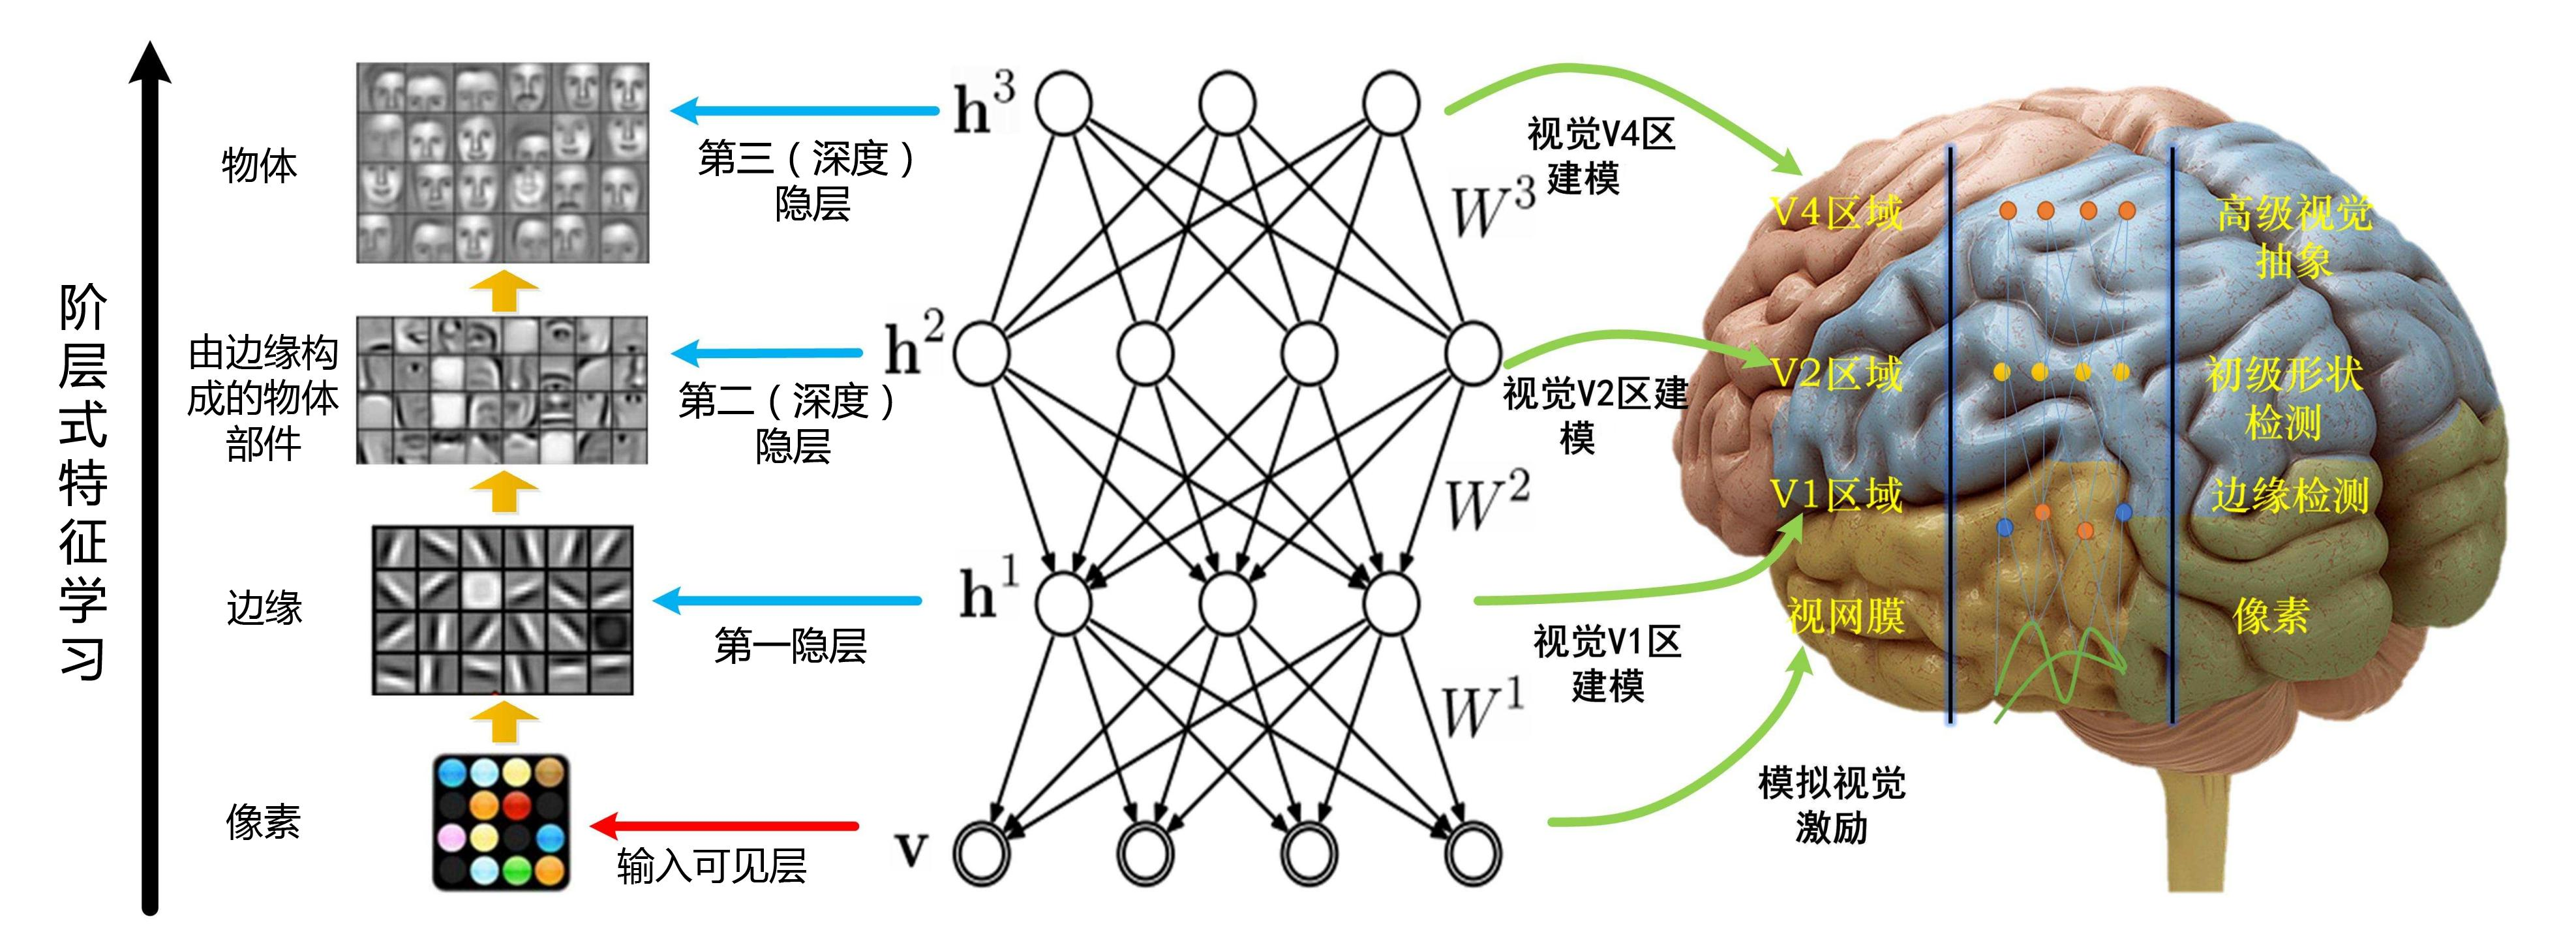
\includegraphics[width=0.9\linewidth]{figures/1-3.jpg} 
\end{center} 
\vspace{-4mm}
\caption{大脑认知和深度学习的关系(示意图)} \label{fig_brain}
\end{figure}

从原始信号摄入开始,接着做初步的处理,然后抽象,然后进一步分析。人类的这种分级认知机制,从机器处理图像的角度来看是一种从低级特征提取到高层特征提取的过程。因此,实现机器像人类一样认知三维形状,图像的特征提取至关重要。如果想要模拟人类视觉系统的分层学习机制,则需要经验丰富的算法设计工程师根据不同的需求,设计出不同层次的特征提取方法,工作量很大并且缺少通用能力。

另一方面,在机器学习领域,目前常用的学习算法例如支持向量机、提升算法,普通的神经网络等都是浅层模型,这些方法的模型通常只有1-3个信息处理层,无法处理现实世界的高度复杂的非线性数据;而人类的大脑的认识、学习是通过多层次的处理来实现的,从而使解决问题的规模可以非常庞大。最近十年间,由于新的神经网络学习方法的研究和计算机能力的提高,克服了以往神经网络层数多而导致的无法训练、过拟合等问题,从而使深度学习得到了快速的发展。最新的研究成果表明,通过深度学习,能够让计算机生成较高层次的语义信息,因此能够填补底层特征和高层语义之间的鸿沟,所以能够极大地提升人工智能的程度。

深度学习已广泛应用于自然语言处理,语音识别,计算机视觉等诸多领域,并展示出了非常优异的性能\cite{Krizhevsky2017ImageNet, He2015Delving, Mnih2015Human}。Dahl等人\cite{Dahl2012Context}提出了一种融合隐马尔科夫模型的混合深度网络,并且在语音识别方面获得巨大成功,在非常具有挑战的数据库上获得了理想的识别精度。Lee等人\cite{Honglak2009Convolutional}使用了卷积深度置信网络来提取图像的阶层特征,在几个图像数据库上都获得较好的识别率。Nitish等人\cite{Srivastava2012Multimodal}提出了多模态的深度学习方法,他们使用了两个深度置信网络来对图像数据和文本标签数据进行建模,并在两个深度网络的上层构建了一个联合表达层来表达这两种数据的关联性。与传统的支持向量机方法相比,该方法能够充分利用多种来源的信息,因此能够获得更高的性能。Kae等人\cite{Kae2013Augmenting}提出了一种融合CRF和玻尔兹曼机的图像标签方法,通过这种融合使深度学习方法提高了结构学习能力。

\section{论文的研究内容及贡献}
目前深度学习(Deep Learning, DL)已经广泛应用于各个领域,可是在三维形状领域目前还不成熟。对三维形状识别检索领域的不断探索,能够不断拓宽深度学习在三维形状分析领域的应用,不断提高三维形状的识别精度,使其更好的服务于社会生产中去。具体来说,论文的贡献如下:

\begin{itemize}
\item 结合多模态融合的思想,首次提出了结合CNN、CDBN、DBN、RBM的多层神经网络的多模态信息融合方法,从而得到具有强表达性质的三维形状特征。
\item 提出了利用获取三维形状视觉信息具有序列化时空信息,提出了基于CNN、LSTM的三维形状识别方法
\end{itemize} 

\section{论文结构安排}

第一章绪论部分介绍了本文的研究背景及意义,说明了本文的研究内容和主要贡献。

第二章详细分析了目前深度学习技术在三维形状应用的最新进展。

第三章详细介绍结合CNN、CDBN、DBN、RBM的多层神经网络的多模态信息融合方法。

第四章详细介绍了基于CNN、LSTM的三维形状识别方法。

第五章对本文工作做了总结,并对后续工作进行了展望。
